\documentclass{article}

\usepackage{graphicx}
\usepackage{tikz}
\usepackage{tikzsymbols}
\usetikzlibrary{calc,patterns,shapes.geometric}
\pagestyle{empty}
\usepackage[margin=0pt]{geometry}
\geometry{papersize={14in,12in}}

\def\centerarc[#1](#2)(#3:#4:#5){\draw[#1] ($(#2)+({#5*cos(#3)},{#5*sin(#3)})$) arc (#3:#4:#5);}

\begin{document}
	\begin{figure}
		\centering
		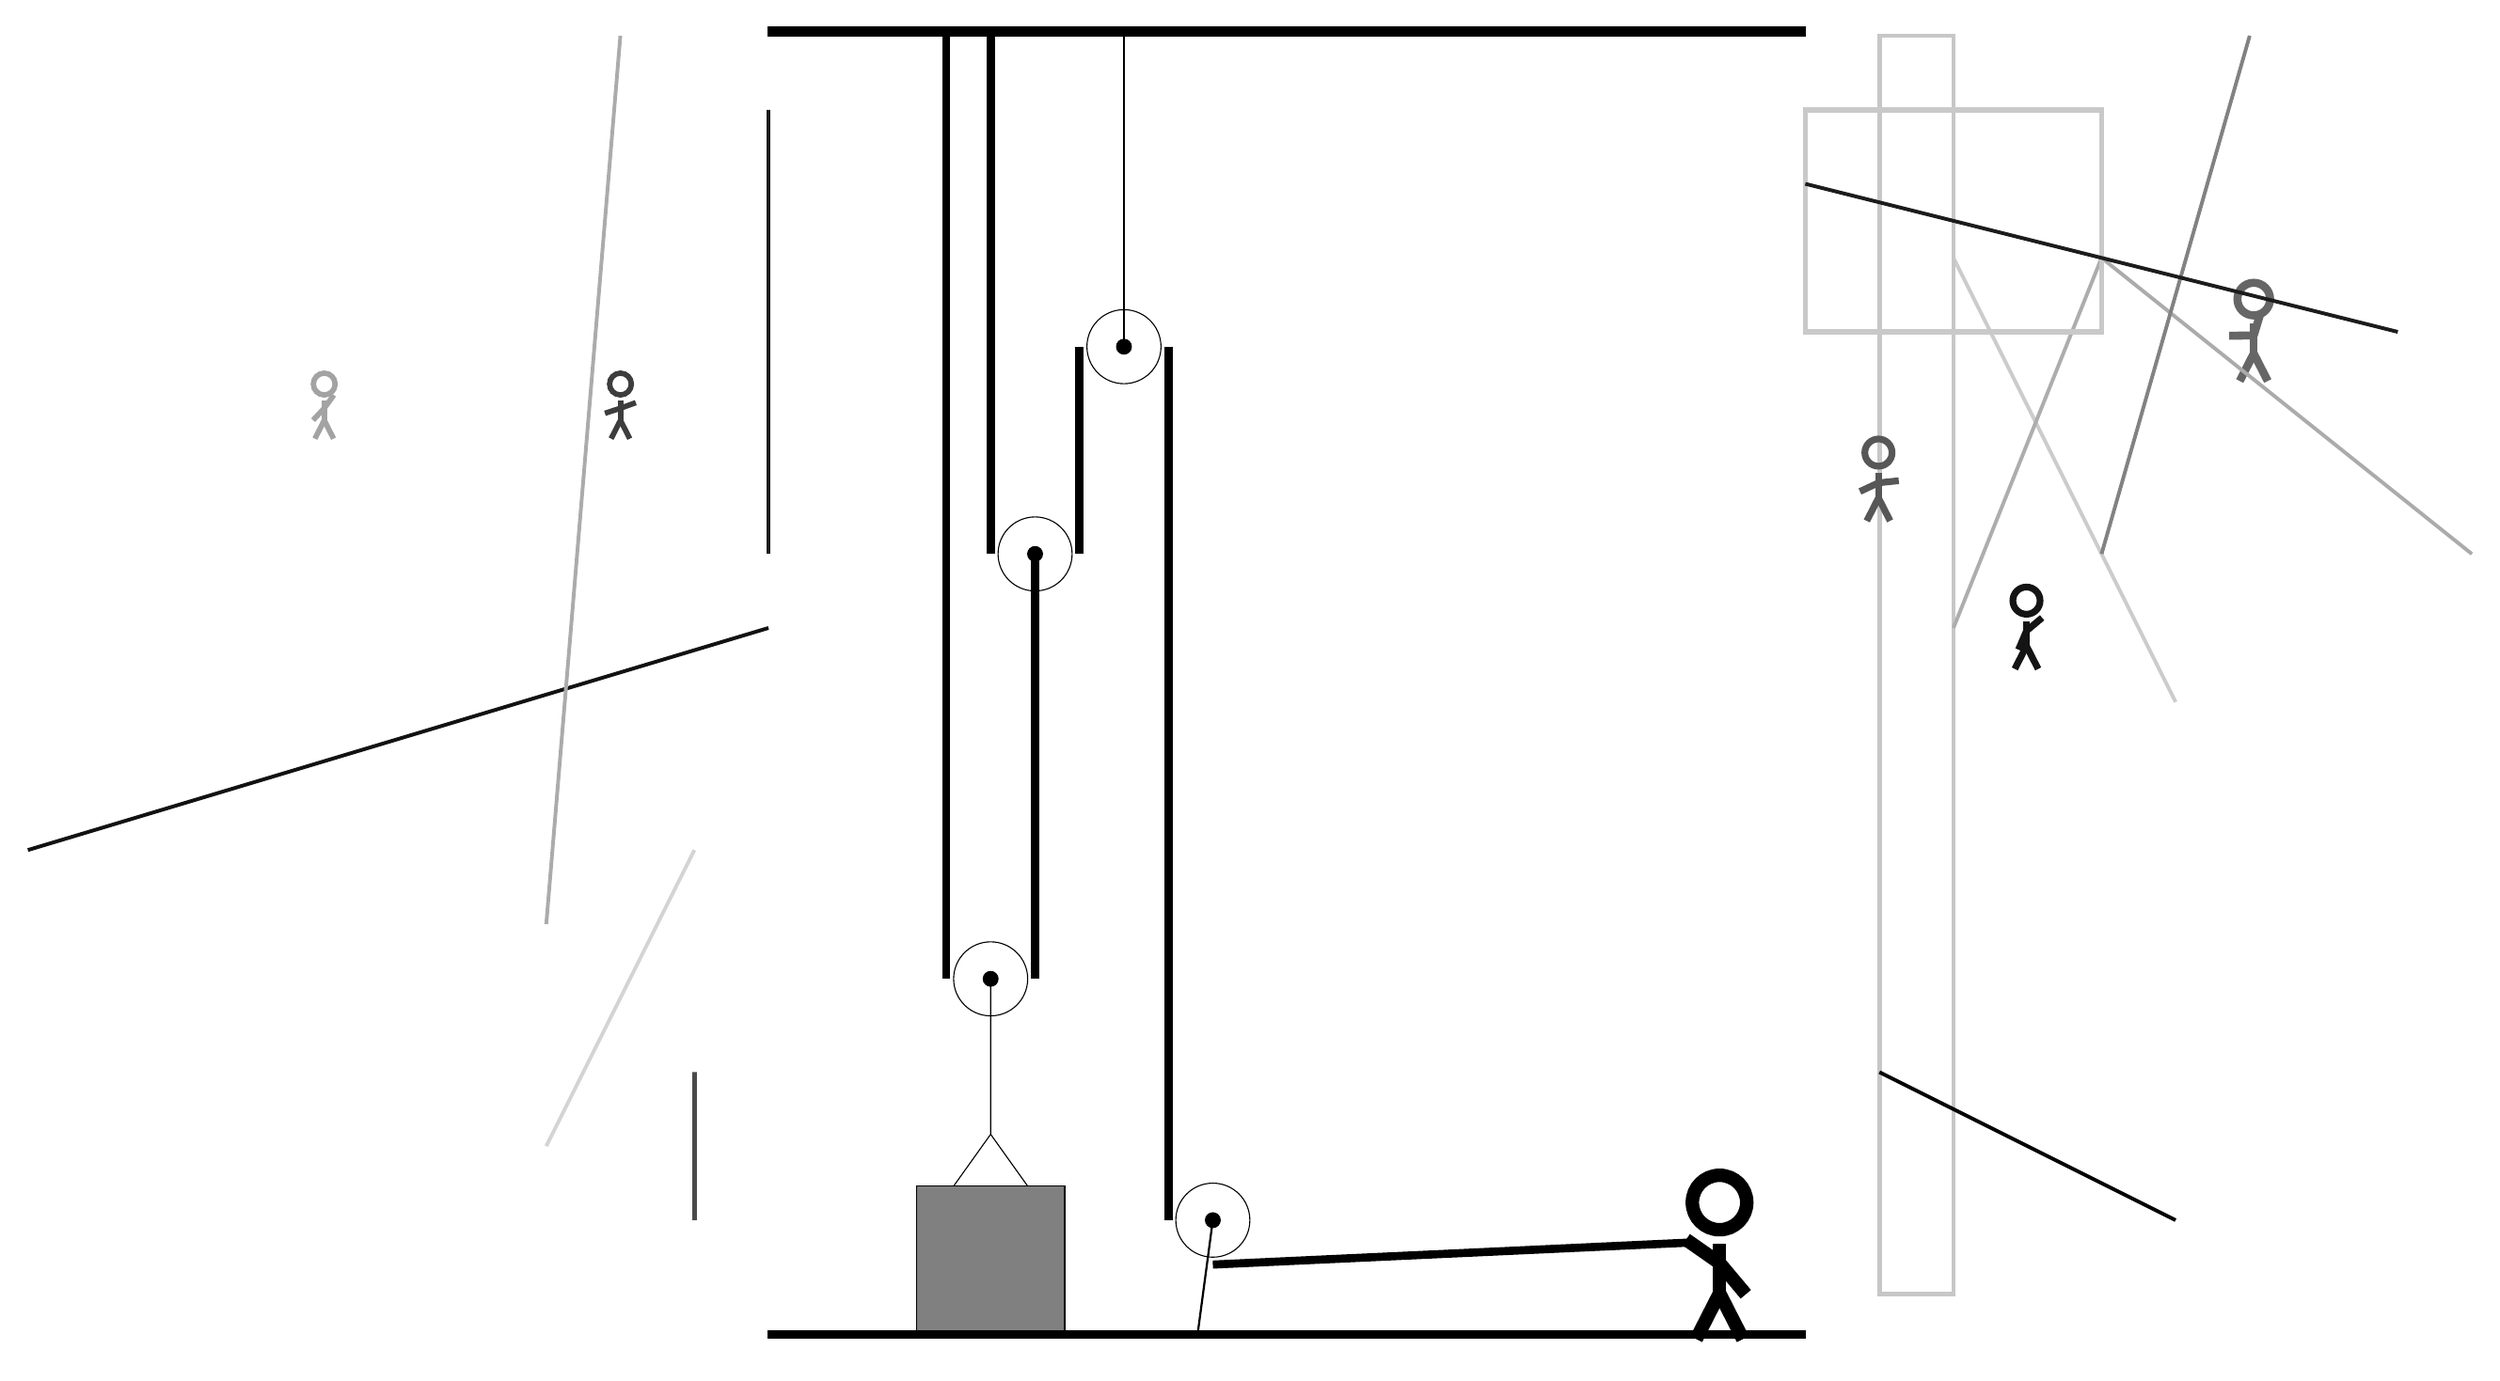
\begin{tikzpicture}
			%%%%% START %%%%%
			
			\draw[fill=black] (-2, 14) rectangle (12, 14.125);
			
			\draw (1, 1.26) circle (0.5);
			\draw[fill=black] (1, 1.26) circle (0.1);
			
			\draw (1.6, 7.0) circle (0.5);
			\draw[fill=black] (1.6, 7.0) circle (0.1);
			
			\draw (2.8, 9.8) circle (0.5);
			\draw[fill=black] (2.8, 9.8) circle (0.1);
			\draw[thick] (2.8, 9.8) -- (2.8, 14);
			
			\draw (4.0, -2) circle (0.5);
			\draw[fill=black] (4.0, -2) circle (0.1);
			\draw[thick] (4.0, -2) -- (3.8, -3.5);
			
			\draw[line width=0.5mm, color=black!93](-2, 6) -- (-12, 3);
			
			\node[line width=0.6mm, color=black!36] at (-8, 9) {\Strichmaxerl[4][47][54]};
			\node[line width=0.5mm, color=black!76] at (-4, 9) {\Strichmaxerl[4][18][20]};
			\draw[line width=0.7mm, color=black!71] (-3, 0) rectangle (-3, -2);
			
			\node[line width=0.6mm, color=black!92] at (15, 6) {\Strichmaxerl[5][67][40]};
			\draw[line width=0.5mm, color=black!20](17, 5) -- (14, 11);
			
			\node[line width=0.4mm, color=black!60] at (18, 10) {\Strichmaxerl[6][1][73]};
			\draw[line width=0.5mm, color=black!89] (-2, 13) rectangle (-2, 7);
			\draw[line width=0.6mm, color=black!22] (14, 14) rectangle (13, -3);
			
			\draw[line width=0.5mm, color=black!33](16, 11) -- (21, 7);
			\draw[line width=0.5mm, color=black!49](16, 7) -- (18, 14);
			\draw[line width=0.5mm, color=black!32](14, 6) -- (16, 11);
			\node[line width=0.5mm, color=black!66] at (13, 8) {\Strichmaxerl[5][25][6]};
			
			\draw[line width=0.5mm, color=black!33](-4, 14) -- (-5, 2);
			\draw[line width=0.7mm, color=black!21] (12, 13) rectangle (16, 10);
			\draw[line width=0.5mm, color=black!17](-3, 3) -- (-5, -1);
			
			\draw[line width=0.5mm, color=black!99](13, 0) -- (17, -2);
			\draw[line width=0.5mm, color=black!89](12, 12) -- (20, 10);
			
			\draw (1, 1.26) -- (1, -0.84) -- (0.5, -1.54) -- (1.5, -1.54) -- (1, -0.84);
			\draw[fill=black!50] (0, -1.54) rectangle (2, -3.54);
			\draw[line width=1.1mm] (0.4, 14) -- (0.4, 1.26);
			\centerarc[line width=1.1mm](1, 1.26)(180:360:0.6);
			\draw[line width=1.1mm](1.6, 1.26) -- (1.6, 7.0);
			\draw[line width=1.1mm] (1.0, 14) -- (1.0, 7.0);
			\centerarc[line width=1.1mm](1.6, 7.0)(180:360:0.6);
			\draw[line width=1.1mm](2.2, 7.0) -- (2.2, 9.8);
			\centerarc[line width=1.1mm](2.8, 9.8)(0:180:0.6);
			\draw[line width=1.1mm] (3.4, 9.8) -- (3.4, -2);
			\centerarc[line width=1.1mm](4.0, -2)(0:90:-0.6);
			\draw[line width=1.1mm](4.0, -2.6) -- (10.5, -2.3);
			
			\node at (10.8, -2.5) {\Strichmaxerl[10][-35][-50]};
			
			\draw[fill=black] (-2, -3.5) rectangle (12, -3.6);
			
			%%%%% END %%%%%
		\end{tikzpicture}
	\end{figure}	
\end{document}